\section{\name: System Design}
\label{sec:systemDesign}

%\begin{figure*}[t]
% \centering
% 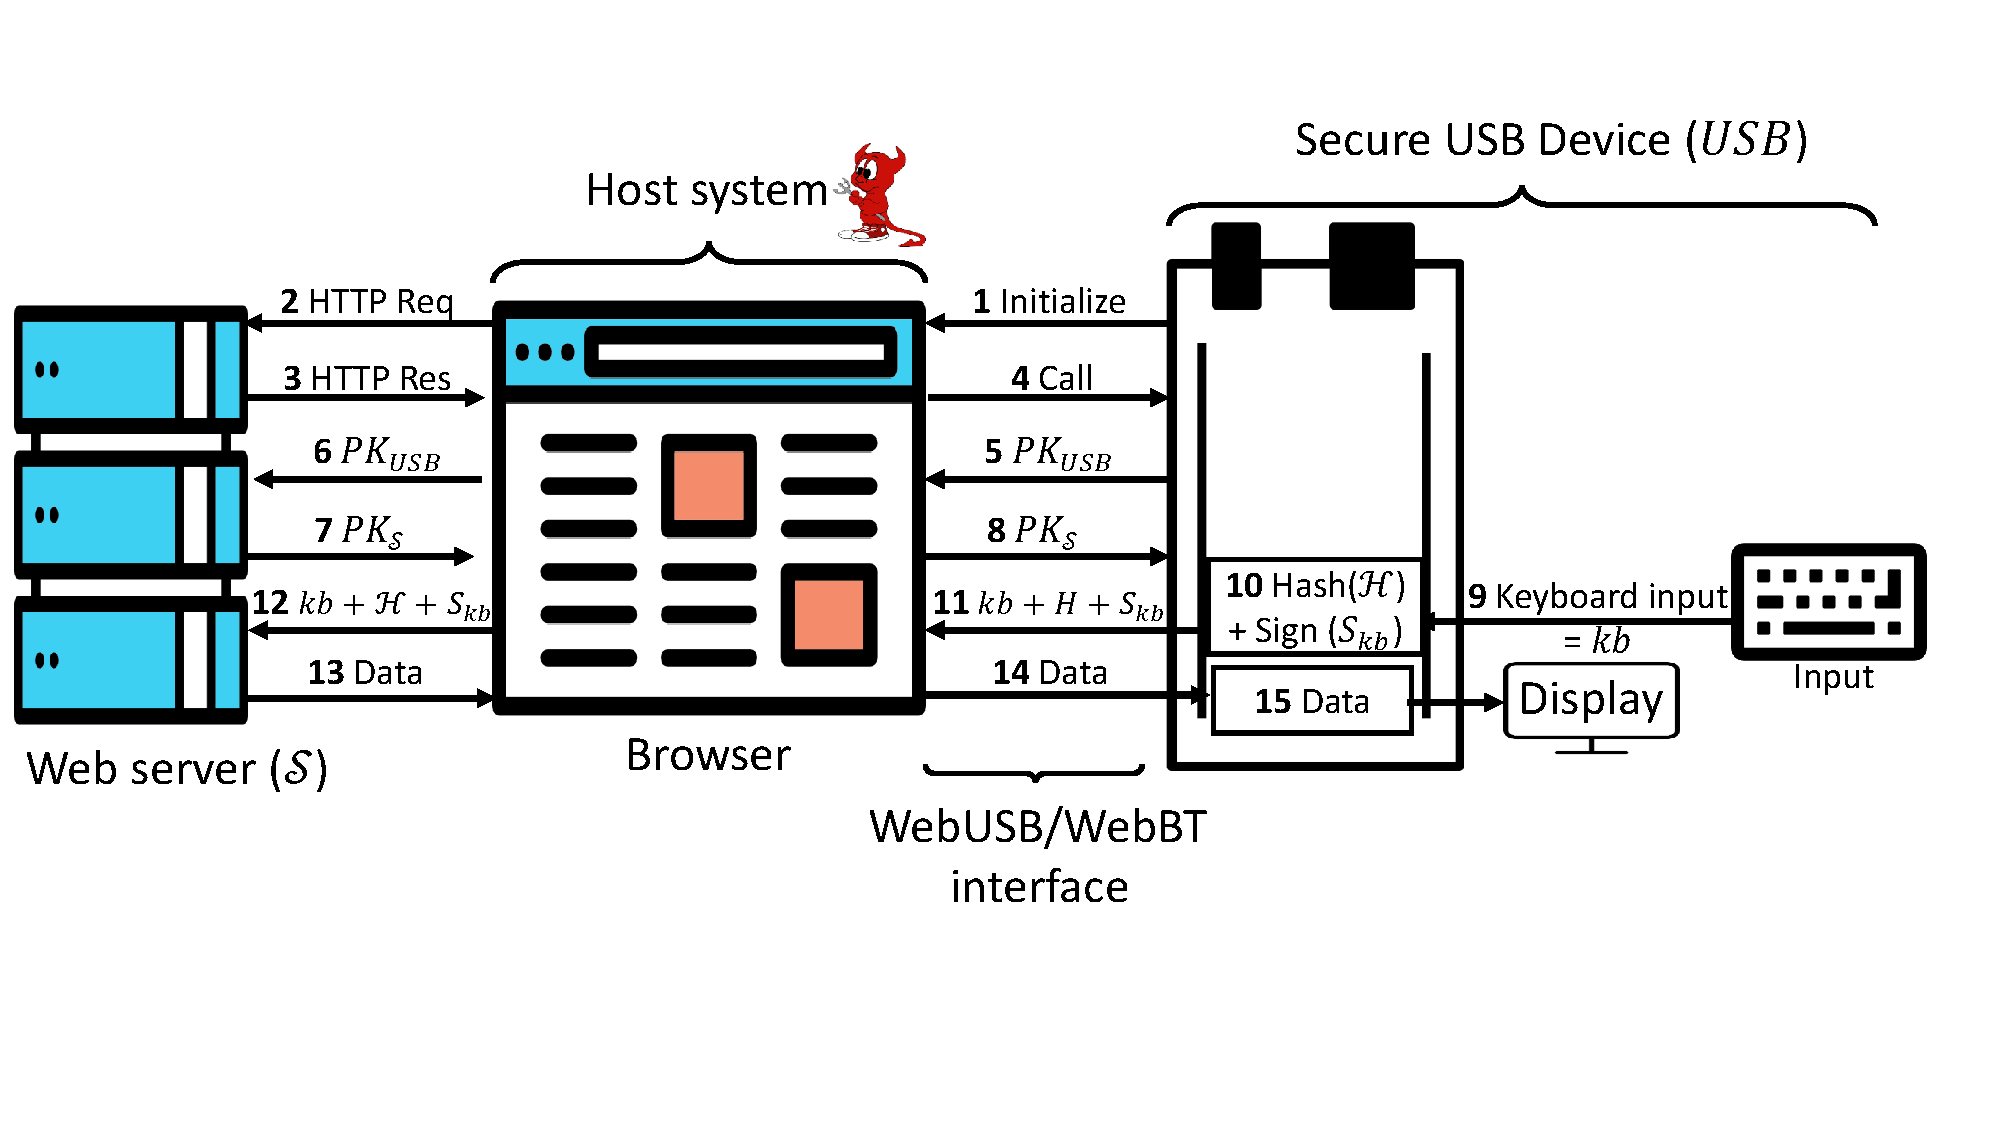
\includegraphics[trim={0 3cm 1cm 1cm}, clip, width=\linewidth]{SystemDesign_auth_ip.pdf}
% \caption{System design of \name. The diagram provides the interaction between the components in the system and the messages that are exchanged between them to establish a secure channel from the \device to the remote server (\server). Steps $1-4$ denotes how the user loads a web page from \server that serves a \js snippet. The \js snippet is written using the \webusb/\webbt API. Steps $5-8$ shows the establishment of the \tls channel using the browser as an untrusted transport. $PK_{USB}$ and $PK_{\mathcal{S}}$ are the public key corresponding to the \device and \server respectively. We assume that \server is trusted and there exists a PKI that we can leverage, Using the PKI, the \device verifies \server's public certificate. Steps $9-12$ shows how the user types a message on the input peripherals that are connected to the \device that transfers the keystrokes securely to \server along with the signature to ensure integrity and authenticity of that input. The \device also houses a primitive display that shows useful information such as the certificate information of \server and confirmation/information related to the service the user is using.}
% \label{fig:systemDesignAuthInput}
%\end{figure*}

\begin{figure*}[t]
 \centering
 %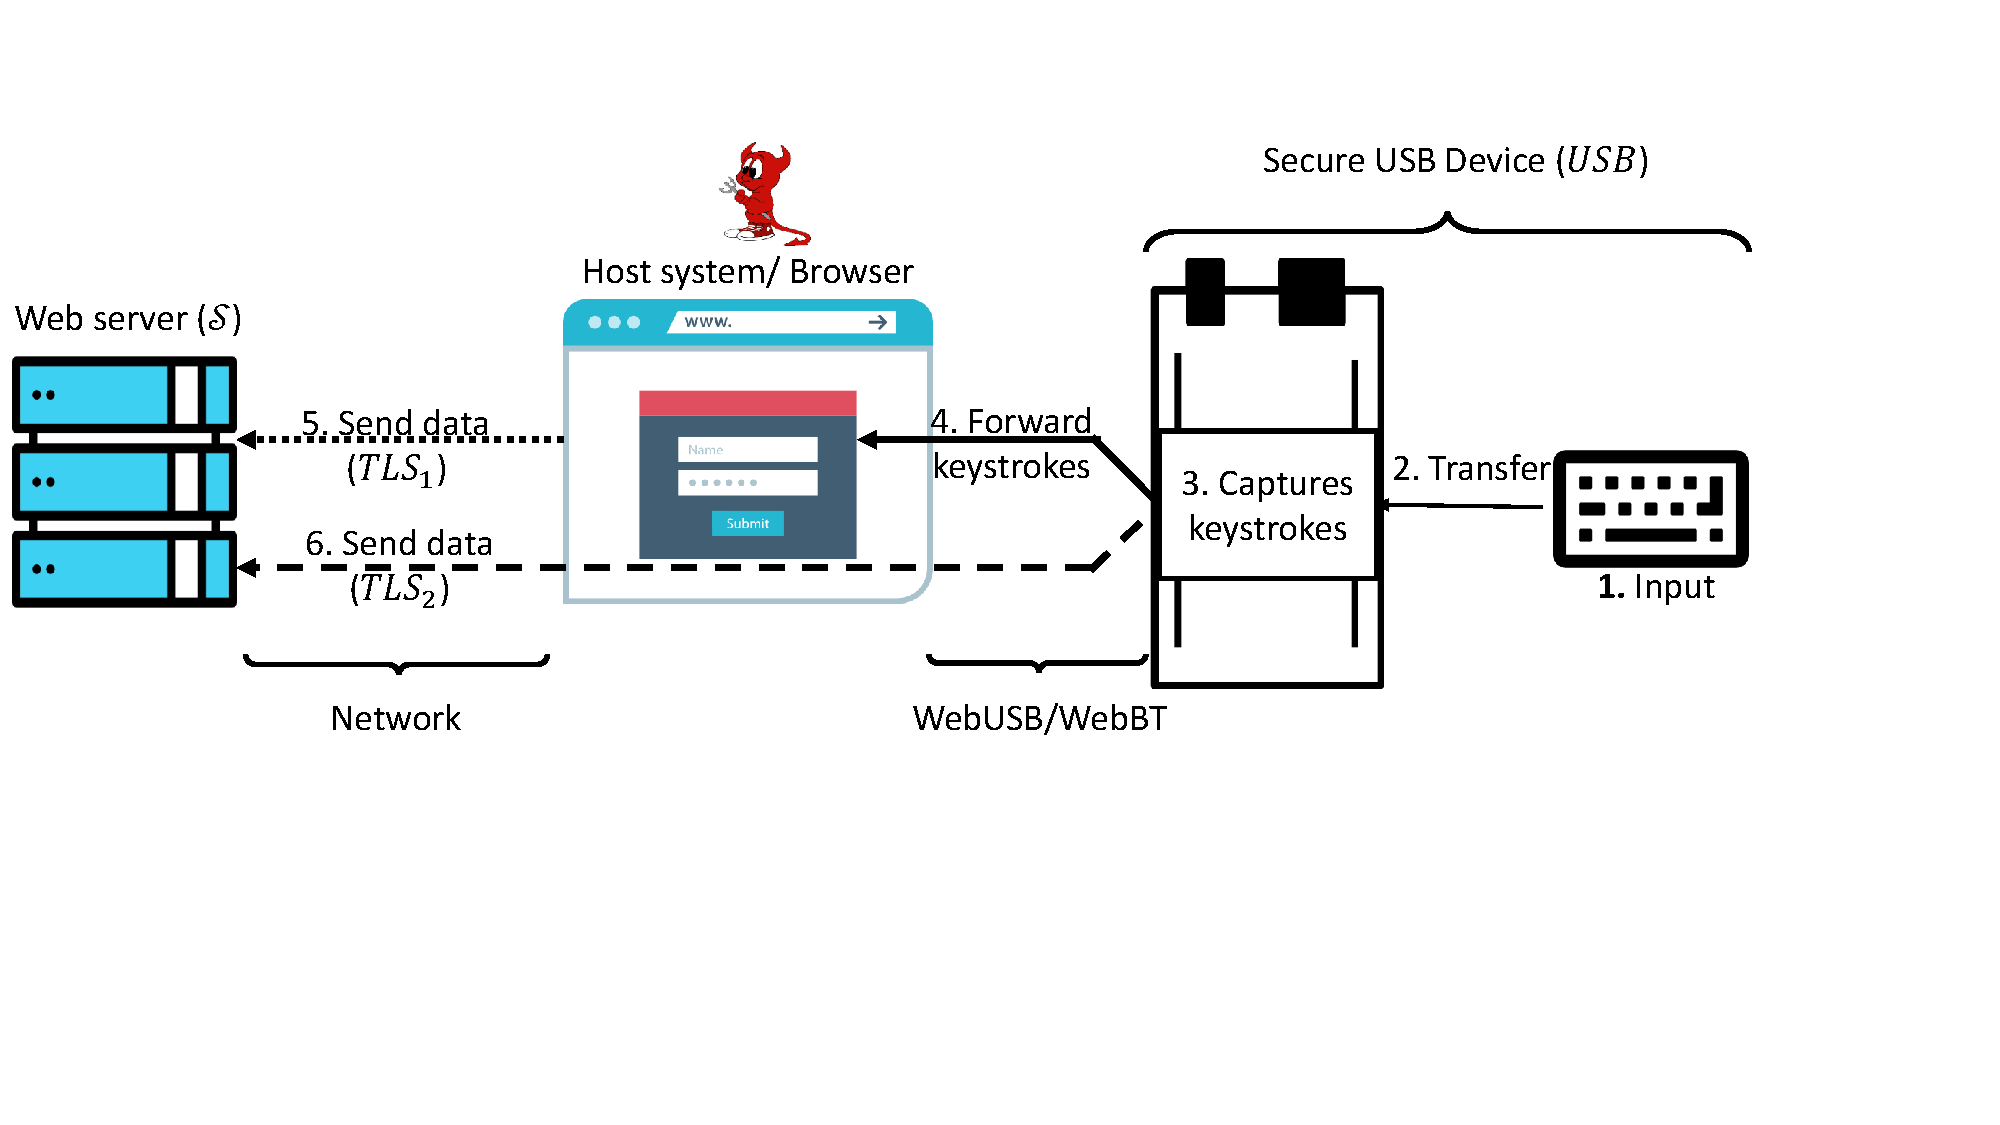
\includegraphics[trim={0 6cm 3cm 1cm},clip,width=\linewidth]{SystemDesign_forms_revised.pdf}
 %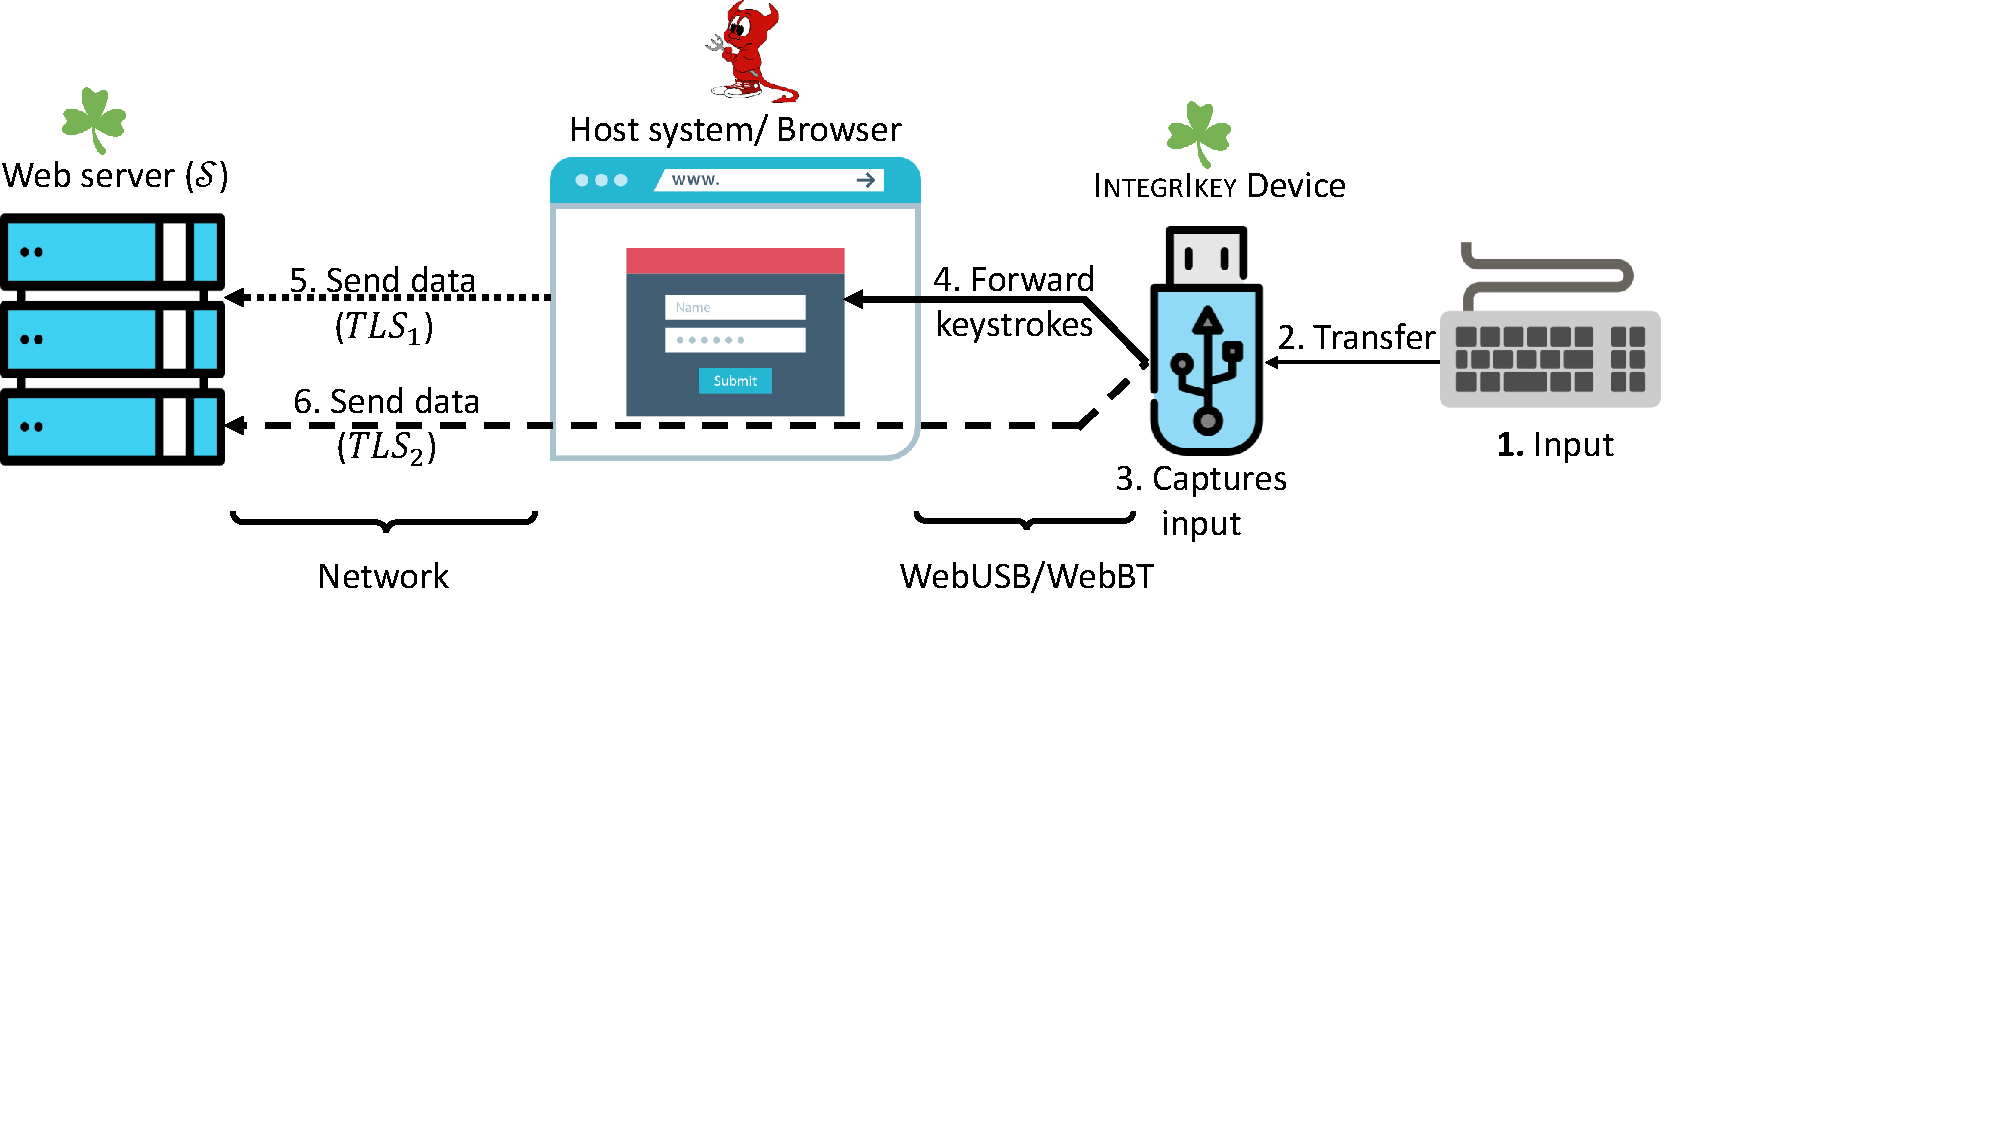
\includegraphics[trim={0 9cm 5cm 0},clip,width=\linewidth]{SystemDesign_forms_revised_1.pdf}
 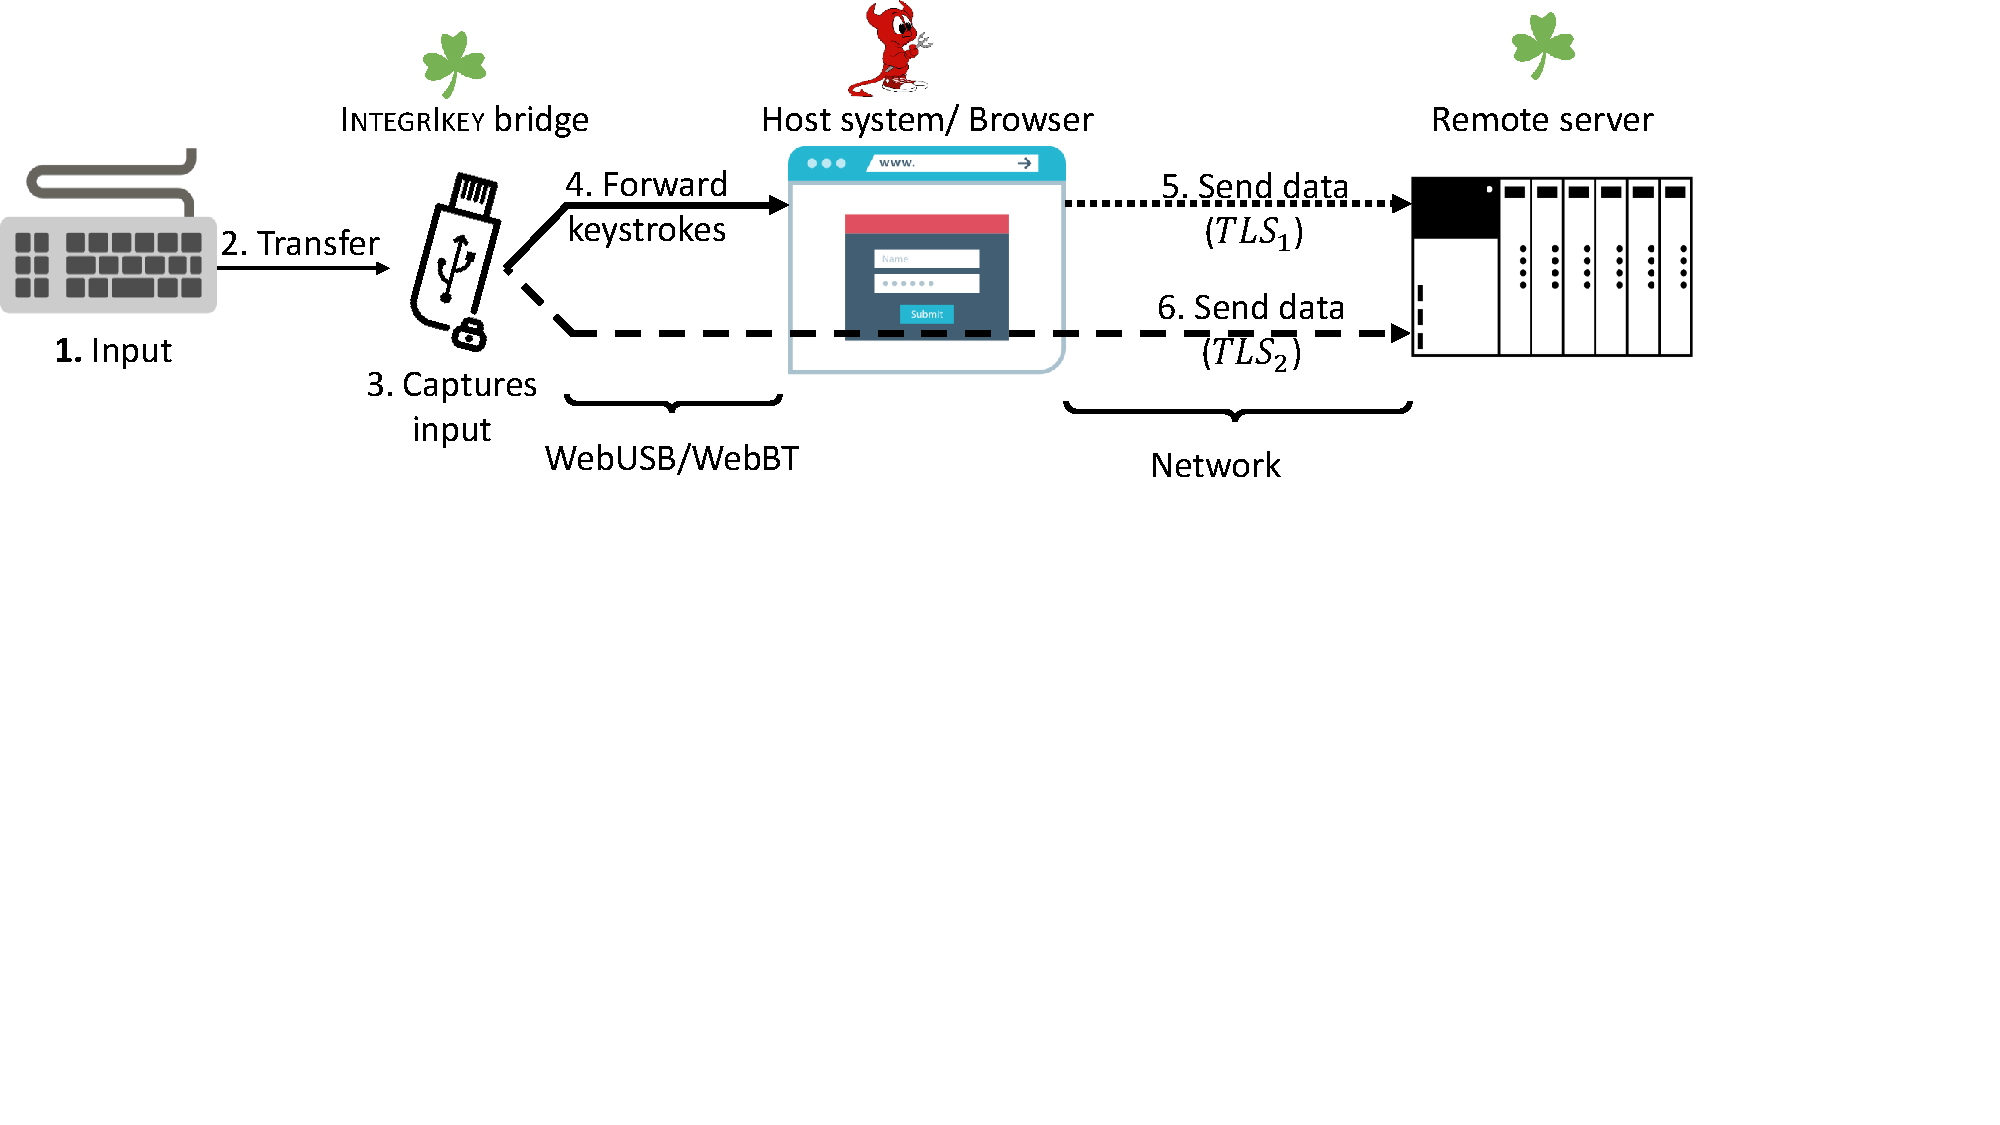
\includegraphics[trim={0 11cm 5cm 0},clip,width=\linewidth]{SystemDesign_forms_revised_2.pdf}
 \caption{\name operation. The \device is connected to the host system over \usb interface and the input peripheral devices such as keyboard is connected with the \device over \usb interface. The user starts the browser and types in the url of the web server. The server will serve the page that contains a script that will instruct the browser (via \webusb) to contact the \device. Two secure connections will be created: an HTTPS ($TLS_1$) connection between the Browser and the Server and a secure connection between the \device and the Server ($TLS_2$). When the user provides the keyboard input, the \device will send this input to the browser (to fill in the web form), and also send it directly via the $TLS_2$ connection to the server\protect\footnotemark. Upon receiving the data from both connections, the server compares them and accepts the input from the browser if it matches the one from the \device.}
 \label{fig:systemDesignForms}
\end{figure*}


In what follows we describe the high-level design of our approach \name that serves as the second factor for the user input. 

\subsection{System Assumptions} 
\label{sec:inputPrivacy:systemModel}

We assume a conventional client-server system which primarily involves three components. The \usb/\bluetooth enabled input peripheral (keyboard, mouse, bulk storage), a host which is a computer/smartphone, that connects to the remote server through a web browser and the remote server where the host is connected. In addition, we assume that the user's browser supports \webusb/\webbt. \webusb is an upcoming standard in development~\cite{webusb} by Google and is currently implemented as a feature in Google Chrome. \webusb allows \js code served from a \https secured page to have direct access to \usb devices. The \webusb API safely exposes USB functionality to the \js code allowing the website to act as a \usb host and communicate with the \usb devices.
%The Universal Serial Bus (USB) is the de-facto standard for wired (even some wireless) peripherals.
%\webusb and \webbt are emerging standards developed primarily by Google which enables browsers to directly communicate with USB devices. \webusb API safely exposes USB functionalities where a Javascript code served by an HTTPS page can query and communicate with USB devices and acts as a USB endpoint.


\subsection{\name: Second factor for Input Integrity}
\name aims to protect the integrity of user's input in highly adversarial settings, where user's host and all intermediary systems that transfer and process user's input to the server are compromised. Furthermore, \name aims to achieve this without changing user's existing behavior and without requiring additional software to be installed on user's host system, therefore, facilitating deployment. 

\name{} achieves this by adding two components to the common client-server: an embedded \device, which captures the user's input (keyboard/mouse) and interacts with the user's browser and therefore with the server via \webusb, and a \name integrity verification server component that detects integrity violations of user's input. 

As shown in Figure~\ref{fig:systemDesignForms}, we assume that the user connects its input peripheral to the \device, and further connects the \device to its host system. This way, the \device acts like a bridge between the input peripheral and the host. These connections can be wired or wireless depending on the interfaces that the host and peripheral expose which will be different in the case of a phone and computer. 

When the user launches her browser and starts a connection to the server, the server will be able to reach the \device via \webusb. The server will, then create two connections, one to the browser (to serve content and take input from the user interface), and the other one to the \device (through the browser via \webusb). The connection to the browser will be protected using \https (\tls). We assume that common user authentication is used. The integrity (and confidentiality) of the communication between the server and the \device will also be protected. This can be achieved in a number of ways, e.g., via pre-shared keys, or via a fresh \tls session. We chose the latter. In \name, the server and the \device exchange public key certificates and establish a \tls channel that will protect their communication. This does not require a setup of a new PKI, \name can also leverage the existing PKI that is used in today's web. The \device can be periodically updated with relevant CA root certificates. 

\footnotetext{TLS connection can be replaced with any authenticated connection, based on digital signatures or shared keys between the \device and the server. For efficiency reasons, it is also possible that the $TLS_2$ only carries the signature of the keystrokes and not the data itself.}

\myparagraph{Key management} We envisioned the key management of the \device in a way that involves minimal user interactions. We rely on existing public key infrastructure (PKI) to manage the keys. \device contains a certificate issued from a trusted issuer and corresponding private key. This certificate is used to establish the dedicated \tls channel between the \device and the remote server. \tls supports client certificate verification that the remote server uses to verify a legitimate \device. 

\myparagraph{Credential transfer} \device can be used to store credential for different services. Upon establishment of a secure channel with the remote server, the \device dispatches the stored credential to the remote server. This requires one-time setup by the user who enters her credential corresponding to services (domain names). This allows \tool to transfer confidential credential information to the remote server without revealing it to the compromised host. Both the private key and the stored credential can be stored in encrypted form inside the \device that can be accessed by the specific user after she provides her PIN.

\myparagraph{User interaction}
When the user enters her input (text, mouse clicks), her input will pass via the \device. The \device will (i) forward the input to the browser so that it is shown on user's screen and sent via \https to the server and (ii) record the input and send it to the server via \device-server TLS connection. The server will then compare what it received from the browser and from the \device. If the input values received from the \device correspond to the values received from the browser, the server will conclude that the input from the browser is legitimate. The server will then indicate to the user (e.g., via an LED indicator on the \device) if the input has been successfully `committed' to the server. This last step is optional and depends on whether such assurance is critical for the application. 
%We provide more details on this in Section~\ref{fig:systemDesignForms}.

In \name the user's experience is largely unchanged. She will interact with the server through the web browser, fill in the forms and submit them to the server in the same manner as in any other system. 

The main steps of the execution of \name are shown on Figure~\ref{fig:systemDesignForms}. 

\begin{enumerate}
\item The user starts a browser and types in the URL of the web server. The server serves a script to the browser that invokes \webusb API, establishing a secure communication channel to the \device. 
  \item The user enters her input into the input peripheral device that is connected to the \device. (steps $1-2$).
  \item The \device captures the keystrokes from the input peripheral (step $3$).
  \item The \device forwards the input to the browser (step $4$). When the user submits the form,  the browser sends the input data to the remote server via the \https ($TLS_1$) channel (step $5$).
  \item The \device further sends the keystrokes directly to the server through the secure channel ($TLS_2$) between the \device and the server (step $6$). 
  \item Upon receiving the data from $TLS_1$ and $TLS_2$, the server compares the data. If the keystroke data from $TLS_1$ matches with the data from $TLS_2$, the server accepts them and sends a feedback signal to the \device via $TLS_2$.
  \item The \device shows the feedback to the user to notify that the proper input is recorded by the remote server. This feedback could be displayed via an attached LCD screen or a LED light.
\end{enumerate}  


\iffalse
\subsection{Security Analysis} 
\label{sec:systemDesign:security_analysis}

We assume a strong attacker that controls host system (that includes the hardware and the operating system), the browser, the cloud/network and any other intermediate component on the path to the server. As the attacker controls the host system, it can manipulate or create fake user input from the browser to the server ($TLS_1$), as well as control the user interface.

We assume that the remote server is a trusted entity and has a public key certificate and corresponding public-private key pair to prove its authenticity by leveraging an existing PKI. The server serves a \js snippet that uses \webusb API to communicate with the \device. The \device has a public/private key-pair and a public key certificate that is used to establish a secure channel ($TLS_2$) with the server. The server can validate such certificates e.g., through a company PKI. The user attaches all her peripheral devices through the \device to eliminate any input manipulation or forged data generated by the malicious host. We assume an authenticated TLS connection setup. Given this, the host cannot impersonate the \device or inject input into the $TLS_2$ channel that was not generated by the user. 
Additionally, the \device also provides a feedback to the user indicating if it has been successfully reprogrammed. In case the \device fails to provide the feedback, the user concludes that the attacker is executing a denial of service attack. Protection against denial of service is outside the scope of this work.

Since the attacker cannot inject messages into the $TLS_2$ channel, the only remaining possibility for the attacker to manipulate the input is to change the user interface (which the attacker controls by controlling the host) such that the user inputs values into the incorrect fields. 
This attack is feasible since the \device only registers the input keystrokes and their sequence, and assumes in which sequence they need to be filled. However, the \device and the server do not know which interface user is currently seeing on the screen. E.g., the fields can be reordered by the attacker. Depending on the end-system and its function, it might happen that these user interface attacks prove detrimental. 

We explore this attack further and propose countermeasures in Section~\ref{sec:fieldSwap}.
\fi

\subsection{Challenges}
\label{sec:systemDesign:challenges}

Given the aforementioned system design of \tool, one can think that the problem of solving integrity of user input while operating on a compromised host is trivial. In contrary, there are many aspects of the system to be solved and all of them poses with technical challenges.

\subsubsection{Easy Setup}
\label{sec:systemDesign:challenges:setup}

One of the most important aspects of \tool is that it involves minimal human involvement to set up. \tool works out-of-the-box as long as the user is using a browser application that is compatible with \webusb API. Additionally, \tool does not rely on any TEE technologies and is compatible with legacy systems. \tool works in a plug-and-play manner where the user connects the \device with the host system and opens the specific web address that points to the remote configuration web page. Another challenge of easy set up is the deployment of \tool in remote servers that operate end systems. This involves adding a \js snippet that uses \webusb API to communicate with the \device and a \tool server-side component that manages the dedicated \tls channel between the \device and the remote server.  


\subsubsection{UI Input Integrity Manipulation Attacks}
\label{sec:systemDesign:challenges:uiAttack}

Previously we described how \device defends against the attacker's manipulation of input values. Now we describe and propose a solution for more sophisticated attacks that compromise the integrity of users' input by manipulating graphical elements on the browser. Our attacker model remains identical to the previous solution, i.e., an attacker that compromises entire host system and the network communications. The malicious host can employ manipulation on the graphical interface elements such as adding extra fields or removing some of the fields. This type of data is effective against inexperienced users who are not properly familiar with the user interface and the specific input fields in a page. Note that when the server serves a specific website, it knows what to expect when the user submits the data into the browser. Therefore, these attacks can be readily detected by the server using the former method due to the discrepancy in the number of input data.  

If the user is experienced with the user interface, a malicious host can orchestrate a more sophisticated attack that swaps the labels of input fields on the served web page. Here, the attacker does not manipulate input values (since these values will be signed by the \device) but instead presents false labels in the web form to the user. The user is then tricked into entering the data into incorrect fields.

The experienced users who are familiar not only with the user interface but also know which data fields to expect are not susceptible to such kind of attacks. However, a malicious host can always show a notification falsely claiming that the server updated the UI elements due to a version upgrade. This way the malicious host can trick even a very experienced user into putting data into a wrong field. Therefore, we can conclude that even the most experienced users are susceptible to the UI manipulation attack that compromises users' integrity. 

One can argue that serving a manual or displaying the template (as security indicator) of the website in a separate display (may be attached with the \device) can prevent UI manipulation attack. However, several existing pieces of research~\cite{197283,41927} show that in practice users tend to ignore security indicators. Therefore, one of the design goals of \tool was not to rely on any security indicator that increases user's cognitive load. \tool rather asks the user to perform a compulsory but a very simple task that associate her input data with the field label which she is seeing on the host's screen. We argue that the additional task that the user performs is extremely simple in nature and does not change the natural user behavior in any significant way.

\begin{figure}[t]
  \centering
    %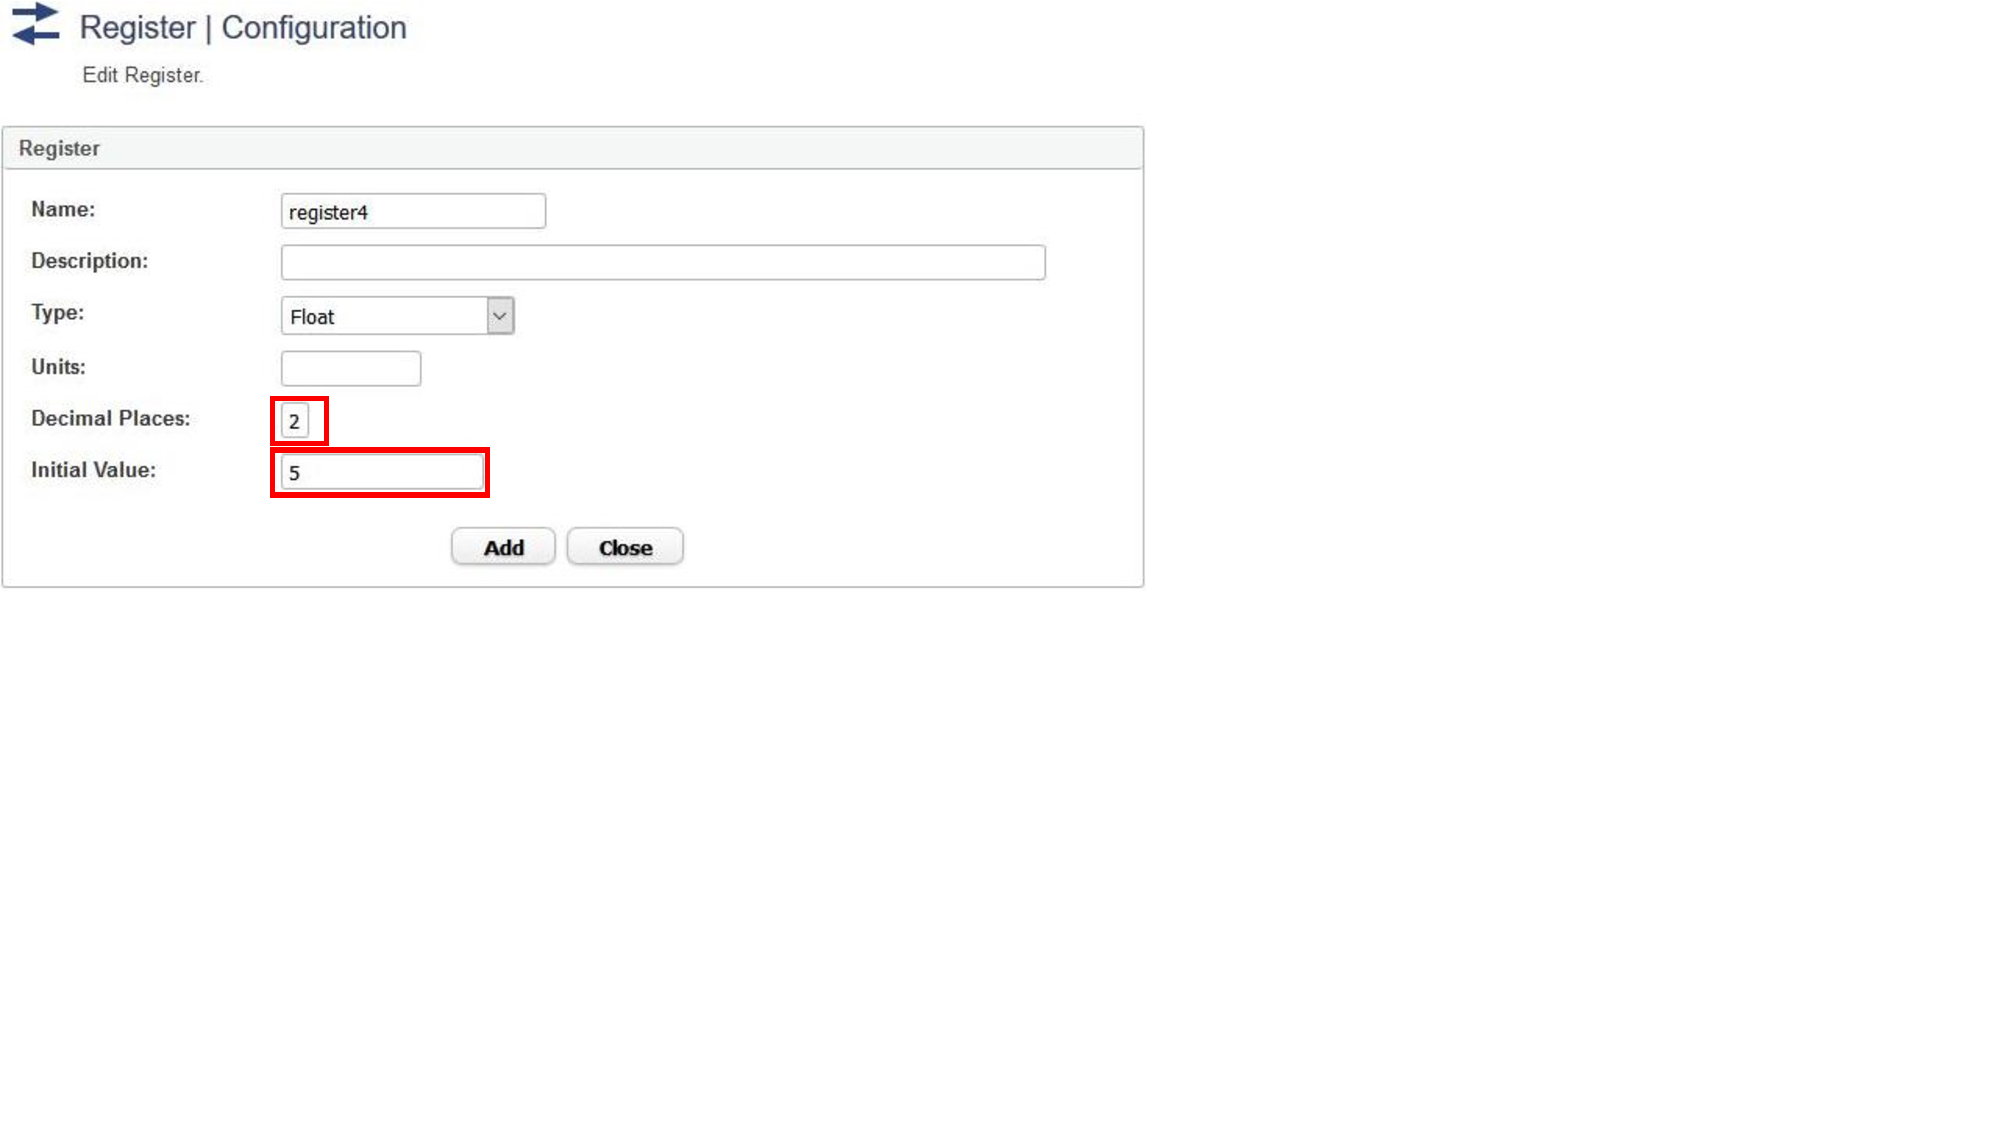
\includegraphics[trim={0 9cm 14cm 0},clip, width=\linewidth]{SwapExample.pdf}
    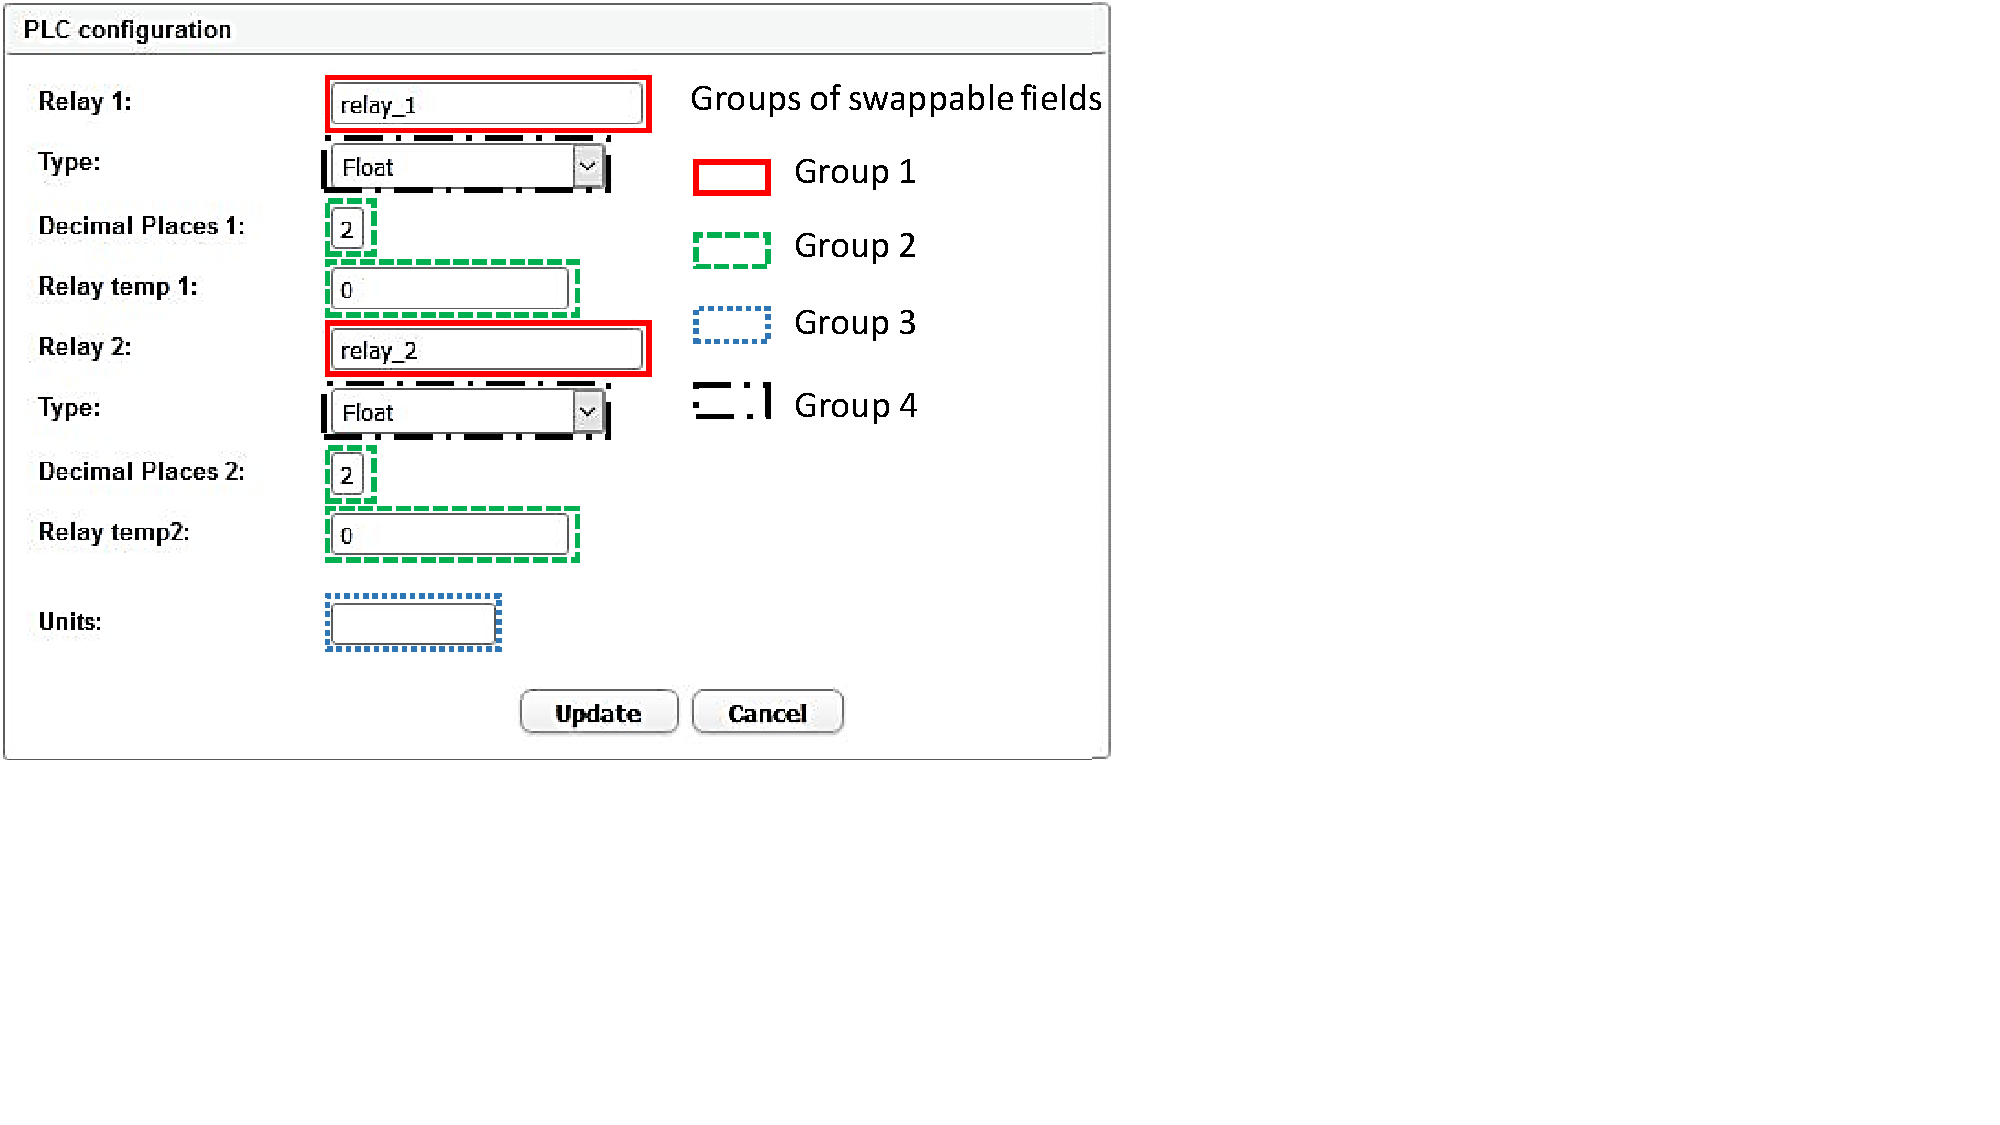
\includegraphics[trim={0 7cm 15cm 0},clip, width=\linewidth]{SwapExample_revised2.pdf}
    \caption{An example of a web-based PLC configuration page where the highlighted fields can be reordered by a malicious host. Note that Relay 1 and Relay 2 are interchangeable, where as Decimal places 1, 2 and Relay temp 1, 2 all are swappable.}
    \label{fig:swapExample} 
\end{figure}


\myparagraph{The attack} Field data types can easily be identical but interchanging the values may change the behavior of the end-system. The \server cannot notice this change since the signed values from the \device will be no different from the values entered through the web form and could be plausible values and entered in a plausible sequence for the served web form. E.g., the attacker can swap the labels of fields 'Decimal Places' and 'Relay temp 1' in the web-form illustrated in Figure~\ref{fig:swapExample}. The user will then enter the values in a sequence ('Relay temp 1', 'Decimal Places'). The server will interpret this as a sequence ('Decimal Places', 'Relay temp 1') since this is the order that should have been imposed by the web form. Since both values are in the expected ranges, the server will not notice the swap, unless these values need to be related (e.g., 'Decimal Places'$<$'Relay temp 1') and the server checks for this relation. However, in many systems, one cannot rely on the end-device logic to check for such consistency and there are many values that will overlap in range but will otherwise be fully independent. Such protections, therefore, do not easily generalize.


\subsection{Alternative Channels} 
\label{sec:systemDesign:alternativeChannel}
In our design of \tool, the dedicated connection that the \device establishes with the server shares the same physical channel as the browser, i.e., the internet connectivity of the host. However, \tool can be configured in such a way that the communication channel of the \device remains separated physically from the host. This can be achieved by using a smartphone application as the \tool bridge. The user connects her peripheral devices with the smartphone, the \tool bridge application communicates with the \usb peripheral device and interprets user inputs. Then the application forms a separate \tls channel using its own network (using WiFi or cellular data). This setup does not require any dedicated hardware device such as \device and leverages existing smartphone of the user. However, it requires trust in the smartphone and additional applications installed in it. Moreover, such setup may not be suited for the industrial PLC operators.


